\problemname{The Clock}

Timla left home at midnight and came back the next midnight, 24 hours later. During that time,
there had been a burglary in the house! 
In the house, Timla has a digital clock that shows the time in 24-hour format with hours,
minutes, and seconds, always six digits. Timla likes to save electricity, so her clock automatically
turns off when no one is in the house. 
To accurately measure how much electricity she saves, she also has a very precise electricity meter.
According to this meter, the clock consumed $N$ energy units during the day she was away. 
Each digit segment in the clock uses one energy unit for every second it is lit. The digits look like
the ones in the picture. For example, 27 digit segments are lit when the time is \texttt{02:41:35}.

\begin{center}
  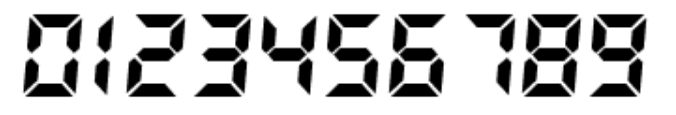
\includegraphics[width=12cm]{illustration.png}
\end{center}


Timla wants to help the police by finding out what time the thief might have broken into the house.
You can see from the shoe prints that the thief went into the house once and out once, so the clock
cannot have turned on and off multiple times. The clock's display always turns on and off at a whole
second and could have turned on as early as \texttt{00:00:00} and turned off at the latest after showing \texttt{23:59:59}.

Write a program that calculates the number of possible times the display could have turned on.

\section*{Input}
Input consists of an integer $N$ ($1 \leq N \leq 3 \cdot 10^6$).

There is at least one time interval during the day when the clock consumed exactly $N$ energy units.

\section*{Output}
Print an integer: the number of different times the clock's display could have turned on.

\section*{Points}
Your solution will be tested on several test case groups.
To get the points for a group, it must pass all the test cases in the group.

\noindent
\begin{tabular}{| l | l | p{12cm} |}
  \hline
  \textbf{Group} & \textbf{Point value} & \textbf{Constraints} \\ \hline
  $1$    & $20$        &  $ N \leq 23 $ \\ \hline 
  $2$    & $20$        &  $ N \leq 200 $ \\ \hline
  $3$    & $20$        &  $ N \leq 5000 $ \\ \hline
  $4$    & $40$        &  No additional constraints. \\ \hline
\end{tabular}



\section*{Explanation of samples}
In the first sample, the clock must have been on for exactly one second. It could have been during \texttt{11:11:17}, \texttt{11:17:11}, or \texttt{17:11:11}.

In the second sample, the only possibility is that the clock was on the entire day, from \texttt{00:00:00} to \texttt{23:59:59}.

In the third sample, there are 3196 possible times when the clock could have started. For example, it could have started at \texttt{20:02:06} and turned off after showing \texttt{20:02:08}.
